\Subsubsubsection{Cálculo Potencias}
Se asumen las siguientes variables para los cálculos de potencias, obtenidas de estadísticas propias de la zona donde se realiza el estudio \cite{ref:weather_bariloche}.
\begin{enumerate}
	\item Duración noche = 12.8 horas.
	\item Duración día = 11.2 horas.
	\item Horas de sol efectivas = 8 horas.
\end{enumerate}

Para el caso de la \rpi, se tiene que su consumo mínimo normal es de $P_{rpi_{min}} = 1.2 \ W$. Sin embargo, para reducir este consumo, se desactivan los puertos de Ethernet y HDMI ya que no se utiliza un entorno gráfico. Esto permite reducir aún más el consumo mínimo. Se estima que la \rspi consume como máximo alrededor de $P_{rpi_{est}} = 1.75 \ W$ en su funcionamiento normal \cite{ref:pot_rpi}. Luego, se tiene que el consumo energético por día es de
\begin{equation}
	E_{sist} = P_{rpi_{est}}\cdot 24 \ hs = 151.2 \ kJ
\end{equation}

Teniendo en cuenta que la batería tiene una tensión de $V_{bat} = 12 \ V$ debe tener una capacidad de almacenamiento equivalente a $T_{reserva} = 4 \ d\acute{\imath}as$ sin recarga \cite{ref:weather_bariloche} y utilizando un coeficiente de seguridad de $\gamma_{bat} = 1.5$, se obtiene
\begin{equation}
	Capacidad_{bat} = \frac{E_{sist}\cdot T_{reserva}\cdot 1000}{V_{bat}\cdot 3600}\cdot \gamma_{bat} = 21 \ Ah
\end{equation}

Por otro lado, para los cálculos del panel solar, se tienen en cuenta que se quiere que en un día de sol promedio se logre abastecer al sistema de su consumo energético normal diario. También, se requiere recargar un $\rho = 0.2$ de la capacidad total de la batería. Además, se considera un coeficiente de seguridad de $\gamma_{panel} = 2$. Es así que se llega a
\begin{equation}
	Pot_{panel} = \left( E_{sist} + \frac{Capacidad_{bat}\cdot V_{bat}\cdot 3600\cdot \rho}{1000}\right)\cdot \gamma_{panel} \cdot  \frac{1000}{60\cdot 60\cdot 8 \ hs} = 23.1 \ W
\end{equation}

\Subsubsubsection{Protección para alimentación \rspi}
Ante la eventual pérdida de energía, en condiciones de funcionamiento normal, es sumamente probable que la memoria SD de la \rspi sea corrompida, dejándola inutilizable. Esto está contemplado en \textit{T-INT-16}, por lo que se diseña un circuito de detección de baja batería, que apaga de manera segura la UP.

Para esto se agrega una bornera, la cual se conecta directamente la batería. De esta manera, se logra medir el nivel de tensión de alimentación, mediante un divisor resistivo.

Comparando este nivel con una tensión de referencia, cuando la batería alcanza un valor inferior al $25\%$ de su capacidad, se cambia el estado de la salida y se apaga la \rspi.
\begin{figure}[H]
\centering
	\begin{subfigure}{0.7\textwidth}
    	\centering
        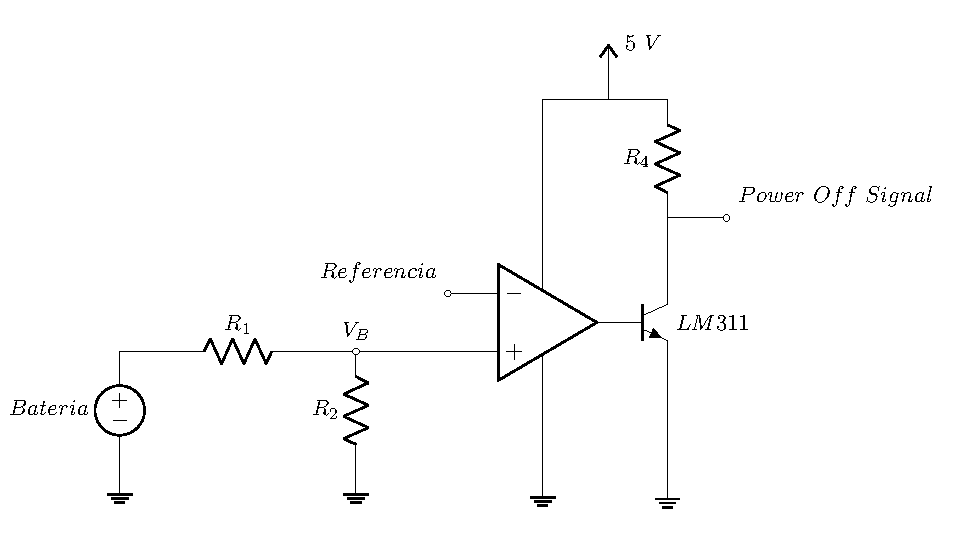
\includegraphics[width=\linewidth, page=1]{ImagenesIngenieria de Detalle/CircuitoProteccion}
		\caption{Comparador de protección.}
	\end{subfigure}      
        
    \begin{subfigure}{0.5\textwidth}
    	\centering
        \includegraphics[width=\linewidth, page=2]{ImagenesIngenieria de Detalle/CircuitoProteccion}				\caption{Sección de referencia.}
    \end{subfigure}
	\caption{Circuito comparador e interruptores.}
	\label{fig:Comp}
\end{figure}

Se realizó la simulación del circuito propuesto, obteniendo los resultados esperados.
\begin{figure}[H]
	\centering
    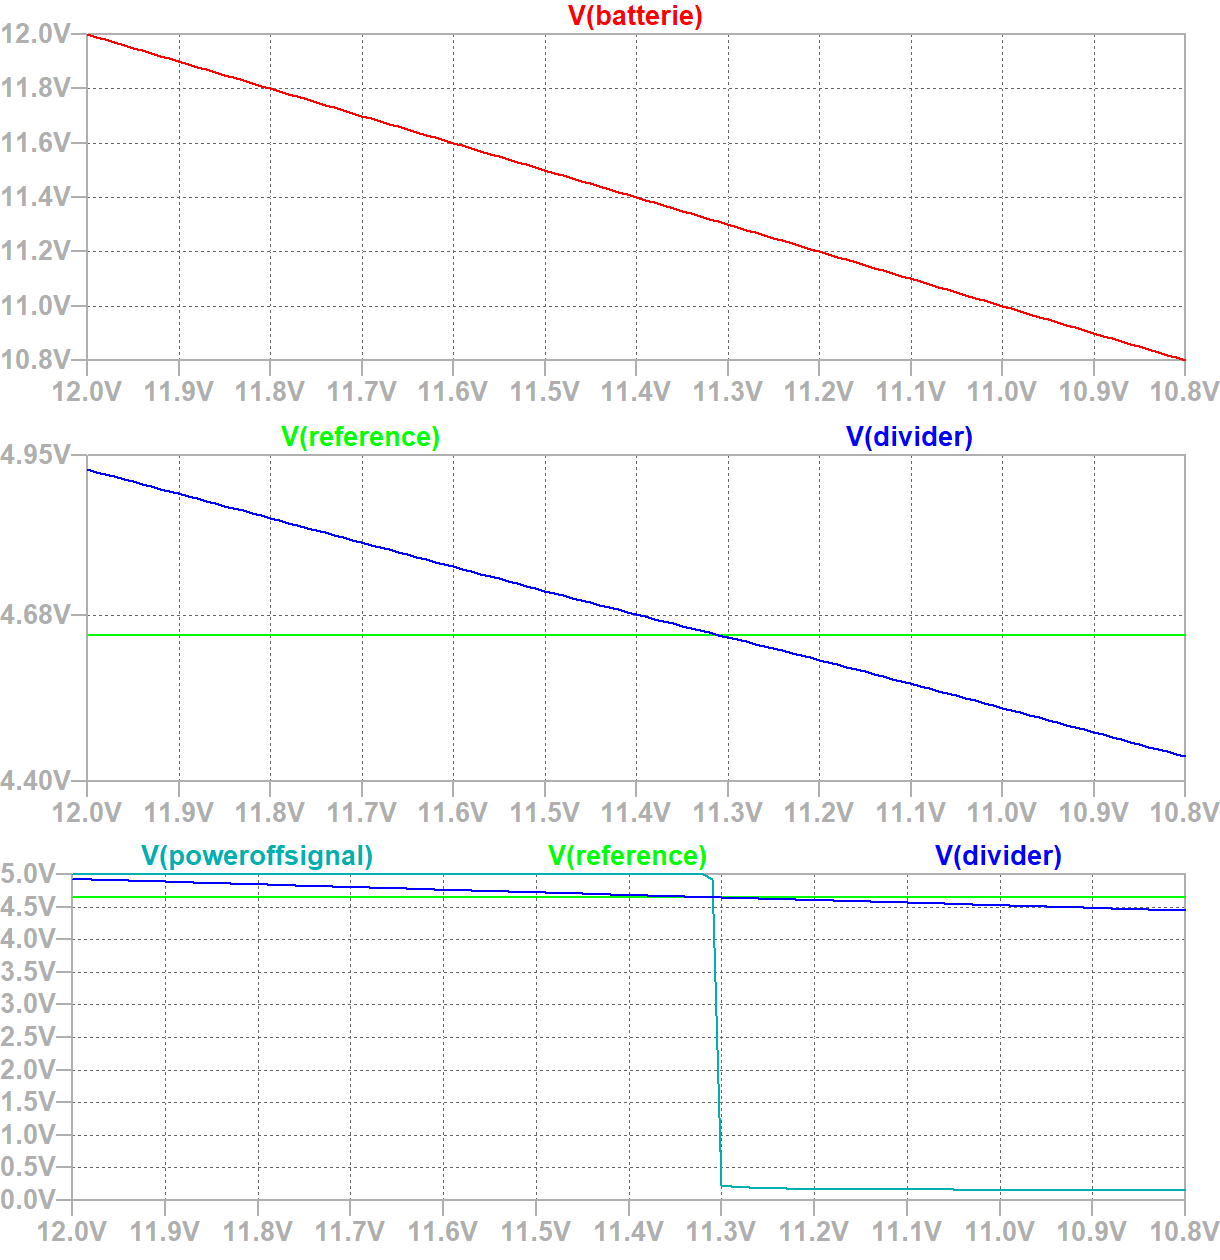
\includegraphics[width=0.9\linewidth]{ImagenesIngenieria de Detalle/Simulation}	
	\caption{Simulación del circuito de protección.}
	\label{fig:sim}
\end{figure}

Se observa como al caer la tensión de la batería, el circuito comparador lo detecta y activa la señal de apagado. Adicionalmente se agregan dos interruptores de apagado y prendido de modo seguro. Estos están destinados para los operarios de instalación y desinstalación, en caso de ser necesarios.

Finalmente, se configura la \rspi para que, con el cambio de tensión del comparador, se efectúen los cambios deseados.
\begin{lstlisting}[language=bash]
sudo nano /boot/config.txt 
dtoverlay=gpio-shutdown,gpio_pin=26,active_low=1,gpio_pull=up
\end{lstlisting} 

\Subsubsubsection{Cálculos circuitales}
Los valores de las resistencias y capacitores utilizados como acondicionamiento de las señales del ESP32-WROOM-S3-1-N4 fueron extraídos de las recomendaciones de las hojas técnicas del dispositivo.

Tanto para el Bus de $I^2C$ como para el DHT22, se calcularon las resistencias de \textit{pull-up}\footnote{En los circuitos digitales, un resistor \textit{pull-up} se utiliza para garantizar que la señal siempre se encuentre en un estado conocido.} de la siguiente manera:
\begin{equation}
	R_p \ = \  \frac{V_{dd}}{I_{R_p}} \ = \ \frac{3.3 \ V}{1 \ mA} \ = \ 3.3 \ k\Omega  
\end{equation}

Para el circuito de protección, se tiene en cuenta que el nivel de tensión de la batería gradualmente disminuye con el uso, mientras que el valor del voltaje regulado de la \rspi no. Esto ocurre siempre y cuando se encuentre en el rango de funcionamiento habitual de la batería.

Es por esto que se decide utilizar esta última tensión para realizar una referencia utilizando una resistencia y un diodo zener de $4.6 \ V$ como el \textit{1N750}. Esta medida es comparada con la de la  batería.

La comparación no es directa, ya que el nivel de tensión de la batería es mayor a los $5 \ V$ provistos por la \rspi. Es así que se emplea un divisor resistivo para bajar el valor. Para ello se tuvo en cuenta que la tensión a la que se baja debe ser mayor a la de referencia para el rango de capacidad de la batería de $25\%$ a $100\%$ y menor caso contrario.
\begin{equation}
R_1 \ +\ R_2 \ = R_{tot}
\end{equation}
\begin{equation}
I_{leak} \ = \ \frac{V_{bat}}{R_{tot}}  = 70 \mu A
\end{equation}
\begin{equation}
R_1 \ = \ \frac{V_{LowBat} \ \cdot \ R_2}{V_{trigger}} \ - \ R_2
\end{equation}

Con estas ecuaciones y teniendo en cuenta que $V_{LowBat} = 11.2 \ V$ y $V_{trigger} = V_{ref} \ = 4.6$, se definen los valores de las resistencias.
\begin{equation}
R_1 = 100 \ K\Omega  \ \ R_2 = 68 \ K\Omega
\end{equation}
Por último, el valor del resistor utilizado para la referencia de tensión se calcula de la siguiente manera:
\begin{equation}
	R_3 = \frac{V_{cc} - V_{zener}}{I_{zener}} = \frac{5 \ V - 4.6 \ V}{8.5 \ mA} = 47 \ \Omega
\end{equation}
\Subsubsubsection{Cálculo de memoria}
Se definen los siguientes valores para cada medición:
\begin{itemize}

	\item Medición temperatura y humedad: 16 $Bytes$ (fecha y hora) + 4 $Bytes$ (humedad) + 4 $Bytes$ (temperatura) = $24 \ Bytes$.
	\item Medición luminosidad: $16 \ Bytes$ (fecha y hora) + $4 \ Bytes$ (luminosidad) = $20 \ Bytes$.
	\item Medición cámara: cada imagen pesa $1.2 \ MBytes$ \cite{ref:rpicam} (considerando una calidad alta).
	\item Información recibida por BT: aproximadamente $2 \ KByte$.
	\item Sistema operativo: $2 \ GBytes$.
	\item Programas y bibliotecas: $2.8 \ GBytes$.
\end{itemize}

De esta forma se tiene el tamaño de las mediciones durante un período de 14 días:
\begin{multline*}
	12 \ \nicefrac{medici\acute{o}n}{hora} \  \cdot \ 24 \ \nicefrac{hora}{d\acute{\imath}a} \  \cdot \ 14 \ d\acute{\imath}a \  \cdot \ \left( \ 24 \  \nicefrac{Bytes}{medici\acute{o}n} \right. \\ \left. + \ 16 \ \nicefrac{Bytes}{medici\acute{o}n} \ + \ 1.2 \ MBytes \right) \ + 2 \ \nicefrac{KByte}{d\acute{\imath}a} \  \cdot \  14 \ d\acute{\imath}a = 4.84 \ GBy
\end{multline*}

Si a esto se le suma el espacio dedicado al sistema operativo, programas y bibliotecas, se obtiene que el tamaño total de memoria necesaria es de aproximadamente $9 \ GBy$.

Además, de lo mencionado en las cuentas, se tiene en cuenta el espacio utilizado por el \textit{overhead} de la base de datos, así también un espacio adicional por si no se visita al nido en el tiempo pactado. Es así que con una memoria de $32 \ GBy$ basta para el proyecto.